La Figura~\ref{fig:anexo_arbol} presenta la estructura del árbol de escenarios utilizado para representar la evolución de la demanda durante los tres períodos del horizonte de planificación.

\begin{figure}[H]
  \centering
  \caption{Árbol de escenarios de demanda de la instancia base}
  \label{fig:anexo_arbol}
  \vspace{0.4em}
  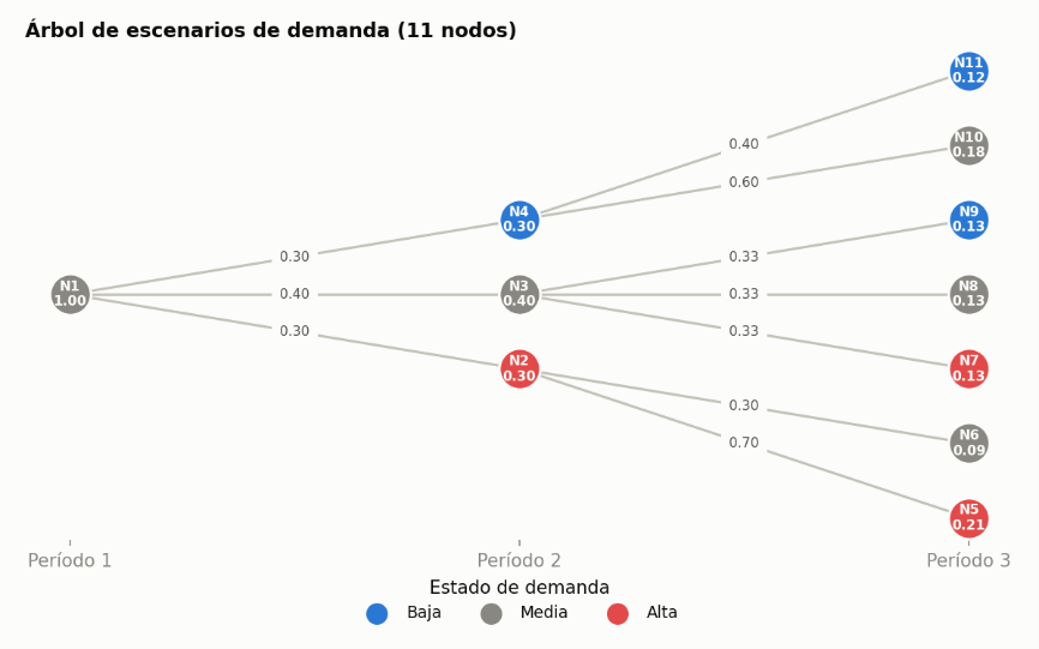
\includegraphics[width=0.75\textwidth]{./figuras/Grafo demanda.png}\par
  \vspace{0.6em}
  {\raggedright \small \textit{Nota.} Estructura compuesta por tres períodos y 11 nodos. Elaboración propia a partir de los datos proporcionados para el proyecto.\par}
\end{figure}

La Figura~\ref{fig:anexo_demanda_esperada} presenta la demanda esperada de cada combinación vino--etiqueta, ponderada por la probabilidad de los nodos terminales del árbol de escenarios.

\begin{figure}[H]
  \centering
  \caption{Demanda esperada por producto}
  \label{fig:anexo_demanda_esperada}
  \vspace{0.4em}
  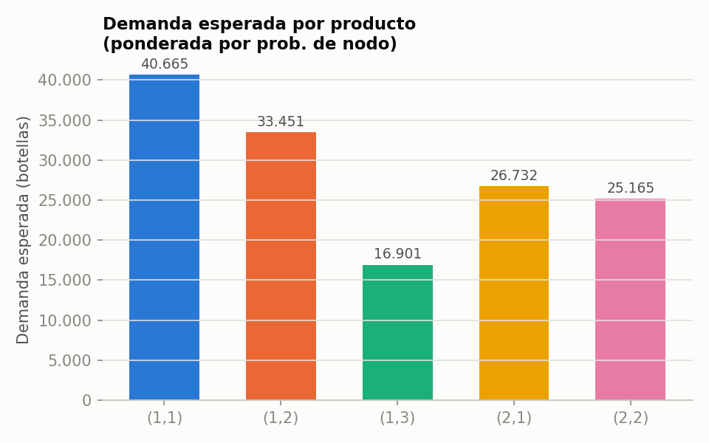
\includegraphics[width=0.75\textwidth]{./figuras/demanda esperada.png}\par
  \vspace{0.6em}
  {\raggedright \small \textit{Nota.} Valores expresados para cada combinación vino--etiqueta y ponderados por la probabilidad de los nodos terminales. Elaboración propia.\par}
\end{figure}

La Figura~\ref{fig:anexo_correlacion} presenta la matriz de correlación de la demanda entre los productos, calculada a partir de los 11 nodos del árbol de escenarios.

\begin{figure}[H]
  \centering
  \caption{Correlación de la demanda entre productos}
  \label{fig:anexo_correlacion}
  \vspace{0.4em}
  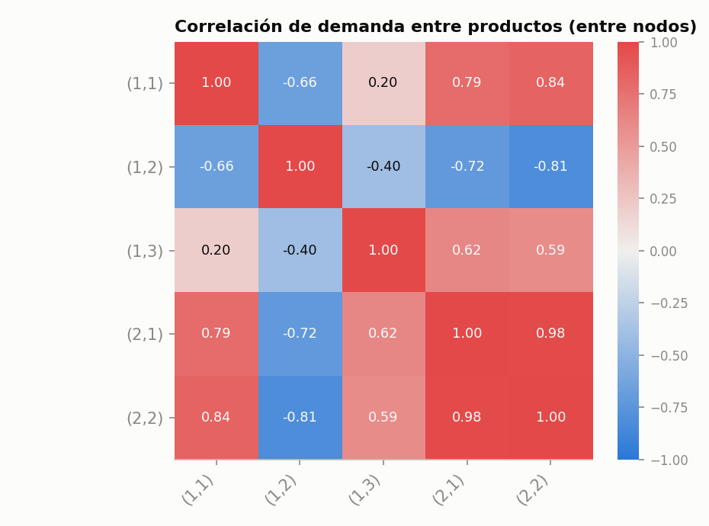
\includegraphics[width=0.75\textwidth]{./figuras/correlación demanda.png}\par
  \vspace{0.6em}
  {\raggedright \small \textit{Nota.} Matriz calculada a través de los 11 nodos del árbol de escenarios. Elaboración propia.\par}
\end{figure}